\documentclass[12pt]{report}
\usepackage[a4paper]{geometry}
\usepackage[myheadings]{fullpage}
\usepackage{fancyhdr}
\usepackage{lastpage}
\usepackage{graphicx, wrapfig, subcaption, setspace, booktabs}
\usepackage[T1]{fontenc}
\usepackage[font=small, labelfont=bf]{caption}
\usepackage{fourier}
\usepackage[protrusion=true, expansion=true]{microtype}
\usepackage[english]{babel}
\usepackage{sectsty}
\usepackage{url, lipsum}
\usepackage{amsmath}
\usepackage{amssymb}

\newcommand{\HRule}[1]{\rule{\linewidth}{#1}}
\onehalfspacing
\setcounter{tocdepth}{5}
\setcounter{secnumdepth}{5}

%-------------------------------------------------------------------------------
% HEADER & FOOTER
%-------------------------------------------------------------------------------
\pagestyle{fancy}
\fancyhf{}
\setlength\headheight{15pt}
\fancyhead[L]{}
\fancyhead[R]{}
\fancyfoot[R]{Page \thepage\ of \pageref{LastPage}}
%-------------------------------------------------------------------------------
% TITLE PAGE
%-------------------------------------------------------------------------------

\begin{document}

\title{ \large \textsc{Assignment 2\\ Mathematical Model
}
		\\ [2.0cm]
		\HRule{1pt} \\
		\LARGE \textbf{\uppercase{STARLING BIRDS MURMURATION}} \\
        \LARGE \textbf{\uppercase{COP290}}
		\HRule{1pt} \\ [0.5cm]
		\normalsize  \vspace*{5\baselineskip}}

\date{}

\author{
		Manish Tanwar 	- 2016CS10363\\ 
        Abhinash Kumar 	- 2016CS10357
		}
\newpage
\maketitle

%-------------------------------------------------------------------------------
% Section title formatting
\sectionfont{\scshape}
%-------------------------------------------------------------------------------

%-------------------------------------------------------------------------------
% BODY
%-------------------------------------------------------------------------------

\section*{Introduction}
\paragraph*{}
This project is to model and simulate starling murmuration.  Objective of this project isto measure from a realistic simulation the average energy spent by each bird, the angular momentum and the force that each bird has to withstand in a typical flight ritual. Starling birds follow number of rules or patterns while foraging. Flocking behavior is one of the most important characteristics shown by starling birds.

\begin{figure}[h!]
    \centering
    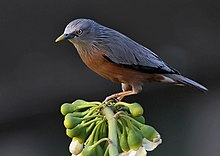
\includegraphics{starling.jpg}
    \caption{A starling bird}
    \label{fig:starling_bird}
\end{figure}


\section*{Steering Rules}
\paragraph*{}
Most of the steering rules are defined by the conditions in the neighbouhood i.e, most of the starling birds mimic their neighbours.
\begin{enumerate}
    \item \textbf{\large{Separation -}}
    \begin{enumerate}
        \item This property helps the boids to be apart and thus avoid from crashing into each other and maintaning distance from other flock mates.
        \item Each boid consider other flock mates in its neighbourhood and applies a repulsive force in the opposite direction.
    \end{enumerate}
    
    \begin{figure}[h!]
    \centering
    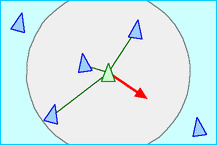
\includegraphics{separation.jpg}
    \caption{Separation}
    \label{fig:Separation}
    \end{figure}
    
    \item \textbf{\large{Alignment -}}
    \begin{enumerate}
        \item It helps in driving boids to head in the same direction with similar velocity .
        \item Boids consider the average velocity of its neighbours and steer in that direction.
    \end{enumerate}
    
    \begin{figure}[h!]
    \centering
    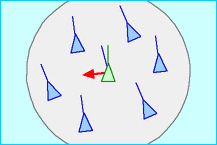
\includegraphics{alignment.jpg}
    \caption{Alignment}
    \label{fig:Alignment}
    \end{figure}
    
    \item \textbf{\large{Cohesion -}}
    \begin{enumerate}
        \item This property helps in keeping boids together as a group.
        \item Each boid moves in the direction of the average position of its neighbours.
        \item Each boid calculates the average position of its neighbours and steer in that direction.
    \end{enumerate}
\end{enumerate}

    \begin{figure}[h!]
    \centering
    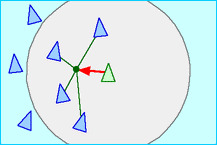
\includegraphics{cohesion.jpg}
    \caption{Cohesion}
    \label{fig:Cohesion}
    \end{figure}


\section*{Mathematical formula}
\begin{enumerate}
    \item \textbf{\large{Velocity -}}
    $$
    \textbf{velocity} = \dfrac{\text{displacement}}{\text{time taken}}
    $$
    \item \textbf{\large{Average velocity -}}
    $$
    \textbf{Avg velocity} = \dfrac{\text{vector sum of the velocities of neighbourhood boids}}{\text{number of neighbourhood boids}}
    $$
    \item \textbf{\large{Work - }}
    $$
    \textbf{Work done} = \text{Force} * \text{time}
    $$\hspace{40mm}\textbf{Total Work done} = \text{Change in Kinetic Energy}$$
    \hspace{10mm} = \Delta \textbf{KE}
    $$
    \item \textbf{\large{Power}}
    $$
    \textbf{Power} = \dfrac{\text{Total Work done}}{\text{total time taken}}
    $$\hspace{70mm} \textbf{OR}$$
    \textbf{Power} = \text{Force} * \text{velocity}
    $$
    
    
\end{enumerate}

\section*{REFERENCES}
\begin{enumerate}
    \item Boids : Background and Update by Craig Reynolds :
    \newline
    \url{https://www.red3d.com/cwr/boids/}
    \item Wikipedia : \url{https://en.wikipedia.org/wiki/Boids}
\end{enumerate}
\end{document}
